\chapter{Fundamentos en la creación de aplicaciones}

\section{Fundamentos de la creación de web-services JAVA}

Para la realización de esta sección se ha tomado como referencia técnica el libro: Fundamentos de programación Java. \cite{javaFun} 

\subsection{Definición}

\begin{shaded}
	\begin{flushleft}	
		Un servicio Web\textit{(web-service)} es una colección de protocolos y estándares que sirven para intercambiar datos entre aplicaciones. La interoperatividad se consigue mediante la adopción de estándares abiertos. 
	\end{flushleft}			
\end{shaded}

Estos servicios proporcionan mecanismos de comunicación estándares entre diferentes aplicaciones, que interactúan entre sí para presentar información dinámica al usuario. Para proporcionar interoperatividad y expansibilidad entre estas aplicaciones, y que al mismo tiempo sea posible su combinación para realizar operaciones complejas, es necesaria una arquitectura de referencia estándar. 
\pagebreak

\subsection{Aspectos comunes de los web-services}

Los aspectos técnicos comunes son: 
\begin{itemize}
	\item Los Servicios Web exponen funcionalidad útil a los usuarios Web mediante un protocolo Web estándar. En la mayoría de casos, el protocolo utilizado es \textbf{Simple Object Access Protocol (SOAP)}. 
	
	\item Los Servicios Web proporcionan un modo de describir sus interfaces con suficiente detalle para permitir a un usuario construir una aplicación cliente para comunicarse con ellos. Esta descripción se proporciona generalmente en un documento XML que responde al nombre de documento\textbf{ Servicios web Description Language (WSDL)}. 
	
	\item Los Servicios Web se registran de modo que los potenciales usuarios puedan encontrarlos. Esto se realiza mediante\textbf{ Universal Discovery Description and Integration (UDDI)}. 
\end{itemize}
	
Aunque la idea de la programación modular no es nueva, el éxito de esta tecnología reside en que se basa en estándares conocidos en los que ya se tiene una gran confianza, como el XML. 

\subsection{Características}
Las principales características son:
\begin{itemize}
	
	\item  Aportan interoperatividad entre aplicaciones de software independientemente de sus propiedades o de las plataformas sobre las que se instalen, permitiendo la interoperatividad entre plataformas de distintos fabricantes mediante protocolos estándar. 
	
	\item  Los servicios web fomentan los estándares y protocolos basados en texto, que hacen más fácil acceder a su contenido y entender su funcionamiento. 

	\item  Al apoyarse en HTTP, los servicios web pueden aprovechar los sistemas cortafuegos sin necesidad de cambiar sus reglas de filtrado. La principal razón para usar servicios Web es que se basan en HTTP sobre TCP en el puerto 80. Dado que las organizaciones protegen sus redes mediante cortafuegos (firewalls) que filtran y bloquean gran parte del tráfico de Internet, cierran casi todos los puertos TCP salvo el 80, que es, precisamente, el que usan los navegadores. Los servicios Web se canalizan por este puerto, por la simple razón de que no resultan bloqueados. 
	
	\item  Permiten que servicios y software de diferentes compañías ubicadas en diferentes lugares geográficos puedan ser combinados fácilmente para proveer servicios integrados. 

	\item  Los servicios web son muy prácticos al aportar gran independencia entre la aplicación que usa el servicio web y el propio servicio. De esta forma, los cambios a lo largo del tiempo en uno no deben afectar al otro. Esta flexibilidad será cada vez más importante, dado que la tendencia a construir grandes aplicaciones a partir de componentes distribuidos más pequeños es cada día más acusada. 

\end{itemize}

\subsection{SOAP}
SOAP es el acrónimo de “Simple Object Access Protocol” y es el protocolo que se oculta tras la tecnología que comúnmente denominamos “Web Services” o servicios web. SOAP es un protocolo extraordinariamente complejo pensado para dar soluciones a casi cualquier necesidad en lo que a comunicaciones se refiere, incluyendo aspectos avanzados de seguridad, transaccionalidad, mensajería asegurada y demás. 

\begin{figure}[H]
	\centering
	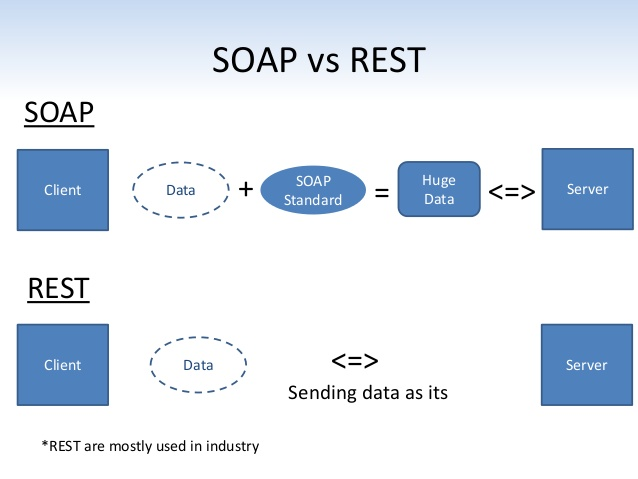
\includegraphics[width=0.7\linewidth]{figuras/soapVSrest}
	\caption{Esquema principal del proyecto Android} 
	\label{fig:soapVSrest}
\end{figure}

\subsection{REST}
REST deriva de \textit{"Representational State Transfer"}, que traducido vendría a ser “transferencia de representación de estado”, más o menos servicio REST no tiene estado \textit{(stateless)}. El estado lo mantiene el cliente y por lo tanto es el cliente quien debe pasar el estado en cada llamada. Si quiero que un servicio REST me recuerde, debo añadirle quien soy en cada llamada. Y lo mismo aplica para el resto de información. 

El no tener estado es una desventaja clara: tener que pasar el estado en cada llamada es, como mínimo, tedioso, pero la contrapartida es clara: esca labilidad. Para mantener un estado se requiere algún sitio (generalmente memoria) donde guardar todos los estados de todos los clientes. A más clientes, más memoria, hasta que al final podemos llegar a no poder admitir más clientes, no por falta de CPU, sino de memoria. 

\subsection{API REST}
En una API REST la idea de “servicio” como tal desaparece. Lo que tenemos son recursos, accesibles por identificadores (URIs). Sobre esos recursos podemos realizar acciones, generalmente diferenciadas a través de verbos HTTP distintos. 

Así, en un servicio web clásico \textbf{(SOAP)} tendríamos un servicio llamado \textbf{\textit{CoffeeService}} que tendría un método \textit{\textbf{GetAll()}} que me devolvería todas los tipos de café. La idea, independientemente de la tecnología usada para consumir el servicio web, es que se llama a un método \textit{\textbf{GetAll()}} de un servicio remoto \textbf{\textit{CoffeeService}}. Del mismo modo para obtener un tipo de café en concreto llamaríamos al método \textit{\textbf{GetById()}} pasándole el id del tipo de café. De ahí que se diga que están orientados a RPC \textit{(Remote Procedure Call – Llamada a método remoto)}. 

Por su parte en un servicio \textbf{(REST)} la propia idea de servicio se desvanece. En su lugar nos queda la idea de un “recurso”, llamémosle “Colección de cafés” que tiene una URI que lo identifica, p. ej. /Coffee. Así, si invoco dicha URI debo obtener una representación de dicho recurso, es decir, debo obtener el listado de todos los tipos de café. 

Para obtener datos de un tipo de café, habrá otro recurso (café) con una URI asociada. Para acceder a uno de sus elementos con una URI tipo /Coffee/123, siendo \textit{123} el ID de la café. 
A la hora de hacer operaciones típicas la URI para acceder es siempre  /Coffee/123 y es el verbo HTTP (GET, POST, PUT, DELETE,...) el que indica cual es la operación que deseamos hacer. 
\begin{figure}[H]
	\centering
	
\includegraphics[width=0.5\linewidth]{figuras/webservice}
	\caption{El conjunto de los Servicios web} 
	\label{fig:webservice}
\end{figure}

\subsection{La elección}
Los servicios web SOAP terminan siendo un monstruo con muchas capacidades pero que en la mayoría de los casos no necesitamos. Por su parte REST es simple. REST no quiere dar soluciones para todo y por lo tanto no pagamos con una demasiada complejidad una potencia que quizá no vamos a necesitar. Así que la elección es clara usaremos REST

\pagebreak


\section{Fundamentos de la creación de aplicaciones Android}

Para la realización de esta sección se ha tomado como referencia técnica el libro: Fundamentos del desarrollo de aplicaciones para Android. \cite{android} 

\subsection{Cómo funciona el sistema operativo Android}
Una vez instalada en un dispositivo, cualquier aplicación corre en su propio entorno limitado de seguridad\cite{android}: 
\begin{itemize}

	\item El sistema operativo Android es un sistema multi-usuario de Linux en el que cada aplicación es un usuario diferente.  

	\item Por defecto, el sistema asigna a cada aplicación de una única ID de usuario \textit{(el ID es utilizado únicamente por el sistema y desconocido para la aplicación)}. Establece permisos para todos los archivos en una aplicación para que sólo el ID asignado pueda acceder a ellos.  

	\item Cada proceso tiene su propia máquina virtual, por lo que el código de una aplicación se ejecuta de forma aislada de otras aplicaciones.  

	\item Por defecto, cada aplicación se ejecuta en su propio proceso de Linux, lo inicia cuando alguno de los componentes se ejecuta, a continuación, cierra el proceso cuando ya no se necesita o cuando el sistema debe recuperar la memoria para otras aplicaciones. 
\end{itemize}

Con esto, el SO implementa \textbf{el principio de privilegios mínimos}, que consiste en que cada aplicación sólo puede acceder a los componentes requeridos para hacer su trabajo. Esto genera un entorno muy seguro en el que la aplicación en cuestión no puede acceder a partes del sistema para las cuales no se le ha otorgado permiso. 
De cualquier modo, existen manera para que una aplicación pueda compartir datos con otras aplicaciones, o también que, una aplicación pueda acceder a los servicios del sistema: 
\begin{itemize}
	
	\item En el caso en el que dos aplicaciones compartan el mismo ID, son capaces de acceder cada una a los archivos de la otra. Para ahorrar recursos del sistema, en este caso en el que dos aplicaciones tienen el mismo ID también se pueden organizar para ejecutar en el mismo proceso de Linux y compartir la misma máquina virtual.  
	
	\item Una aplicación puede solicitar permiso para acceder a los datos del dispositivo, tales como los contactos del usuario, el almacenamiento externo (tarjeta SD), cámara, etc. Todos los permisos de la aplicación debe ser autorizados por el usuario durante la instalación.  
\end{itemize}

\subsection{Componentes de las Aplicaciones Android}

Los principales componentes de toda aplicación Android son:
\begin{itemize}
	 
	\item \emph{\textbf{Actividades\textit{(Activities)}: }} Cada pantalla de una aplicación. Utilizan Vistas (Views) como componentes que muestran información y responden a las acciones del usuario 

	\item \emph{\textbf{Servicios\textit{(Services)}: }} Componentes de la aplicación que se ejecutan deforma invisible, actualizando los datos y las Actividades, y disparando Notificaciones. Realizan el procesamiento normal de la aplicación que debe continuar incluso cuando las Actividades de la aplicación no están visibles. 
	
	\item \emph{\textbf{ Proveedores de Contenidos\textit{(Content Providers)}: }}   Almacenes de datos compartidos. Gestionan las Bases de Datos para las aplicaciones. 

	\item \emph{\textbf{Intenciones\textit{(Intents)}: }} Mecanismo que permite el paso de mensajes destinados a ciertas Actividades o Servicios, o a todo el sistema \textit{( Broadcast Intents)}. Exponen la intención de que se haga algo. 
	
	\item \emph{\textbf{Receptores de Broadcast\textit{(Broadcast Receivers)}: }} Los crean las aplicaciones como consumidores de las Intenciones de broadcast que cumplan ciertos criterios. 

	\item \emph{\textbf{Notificaciones\textit{(Notifications)}: }} Mecanismo que permite a las aplicaciones señalar algo a los usuarios sin interrumpir la Actividad en primer plano. 
\end{itemize}

\begin{figure}[H]
	\centering
	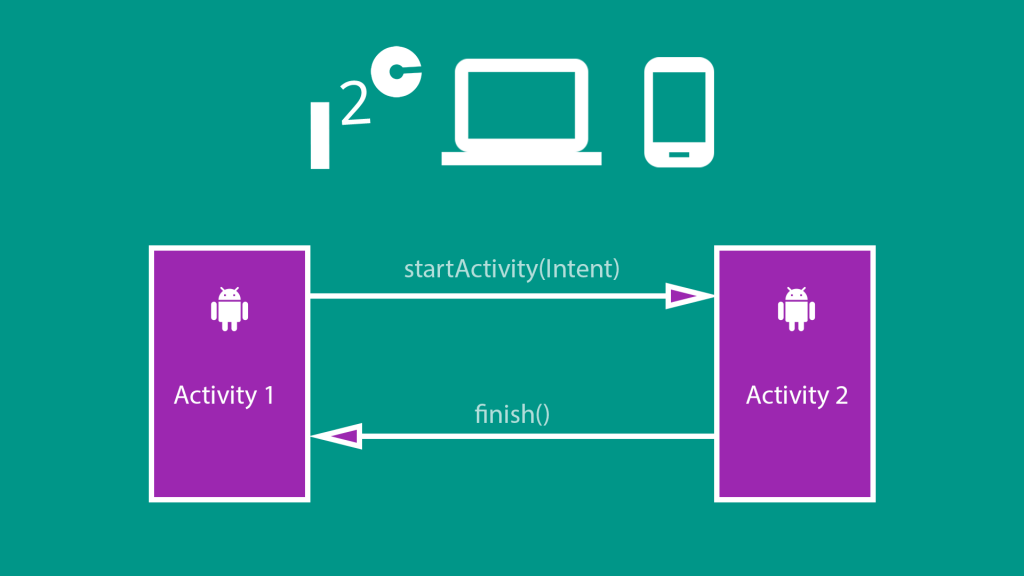
\includegraphics[width=0.8\linewidth]{figuras/activity}
	\caption{Interacción de actividades}
	\label{fig:activity}
\end{figure}



Ademas también existen nuevas implementaciones \textit{(fragmentos, Asíncronos, etc.)} que no vamos a explicar.

\subsection{Manifiesto de una Aplicación Android \textit{(Android manifest)}}

Toda aplicación desarrollada en Android incluye un fichero de Manifiesto, el \textit{\textbf{AndroidManifest.xml}}. Este define la estructura de la aplicación y sus componentes. Incluye un nodo raíz y un nodo para cada uno de sus tipos de componentes. A través de filtros determina como interactuará la aplicacións. 
Algunos de los nodos más importantes son: 
\begin{itemize}
	\item \emph{\textbf{Nodo raíz\textit{(manifest)}: }} Incluye el nombre del paquete de la aplicación. 
	
	\item \emph{\textbf{Nodo aplicación\textit{(application)}: }} Indica los metadatos \textit{(título, icono, tema, etc.)} y contiene los nodos de actividades, servicios, proveedores de contenido y receptores de broadcast. 

	\item \emph{\textbf{Nodo permisos a usar\textit{(uses-permission)}: }}  Declara los permisos necesarios para operar. Estos serán presentados al usuario durante la instalación para que los acepte o deniegue. 

	\item \emph{\textbf{Nodo permisos a proveer\textit{(permission)}: }} Nodo . Define un permiso que se requiere para que otras aplicaciones puedan acceder a partes restringidas de la aplicación. Las otras aplicaciones necesitarán poner un uses-permission en su Manifiesto para utilizar este permiso. 
	
	\item \emph{\textbf{Nodo instrumentación\textit{(instrumentation)}: }} Nodo . Permite definir test de ejecución para las Actividades y Servicios. 
\end{itemize}	

\begin{figure}[H]
	\centering
	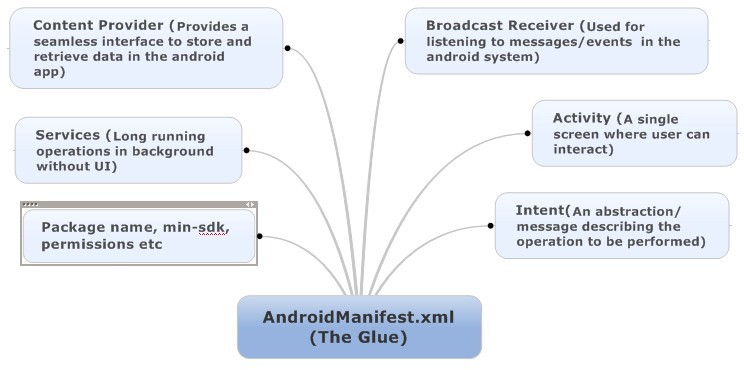
\includegraphics[width=0.95\linewidth]{figuras/androidmanifest}
	\caption{Elementos de un manifiesto Android}
	\label{fig:androidmanifest}
\end{figure}


\subsection{Creación y destrucción de Aplicaciones y Actividades \textit{(Ciclo de vida)}}

Las aplicaciones Android son diferentes a sus homologas en los sistemas operativos tradicionales, en Android sólo hay una aplicación en primer plano que normalmente estará ocupando toda la pantalla. Las aplicaciones estarán formadas por Actividades.
 
Al arrancar una nueva aplicación, pasa a primer plano situando una Actividad encima de la que hubiera, formándose así una pila de actividades. En el momento en el que el usuario presiona el botón “back”, se cierra la actividad en primer plano y recupera la de la cima de la pila. 
Las aplicaciones Android no tienen control ninguno sobre su propio ciclo de vida, esto implica que deben estar pendientes de posibles cambios en su estado y reaccionar como corresponda. En particular deben estar preparadas para su terminación o destrucción en cualquier momento. 
 
Una actividad se puede encontrar en los siguientes estados: 
\begin{itemize}	
	\item \emph{\textbf{Activa\textit{(Running)}: }}  La actividad está encima de la pila, es visible, tiene el foco. Cuando otra actividad pase a estar activa, esta pasará a estar pausada. 
	
	\item \emph{\textbf{Pausada\textit{(Paused)}: }} La actividad es visible pero no tiene el foco. Se alcanza este estado cuando pasa a activa otra actividad transparente o que no ocupa toda la pantalla. Cuando una actividad es tapada por completo pasa a estar parada. 
	
	\item \emph{\textbf{Parada\textit{(Stopped)}: }} Cuando la actividad no es visible. Permanece en memoria reteniendo su estado. Cuando una actividad entra en parada puede ser bueno que salve todos sus datos y el estado de la interfaz de usuario. 

	\item \emph{\textbf{Destruida\textit{(Destroyed)}: }} Cuando la actividad termina, o es matada por el runtime de Android. Sale de la pila de actividades. Necesita ser reiniciada para volver a estar activa. 
\end{itemize}

Y del mismo modo existirán una serie de métodos de transición entre unos estados y otros: 
\begin{itemize}	
	\item \emph{\textbf{onCreate(): }} Se invoca cuando la Actividad se arranca por primera vez. Se utiliza para tareas de inicialización, como crear la interfaz de la Actividad. 
	
	\item \emph{\textbf{onStart(): }} Se invoca cuando la Actividad va a ser mostrada al usuario.
	
	\item \emph{\textbf{onResume(): }} Se invoca cuando la Actividad va a empezar a interactuar con el usuario. 
	
	\item \emph{\textbf{onPause(): }} Se invoca cuando la actividad va a pasar al fondo porque otra actividad ha sido lanzada para ponerse delante. Se utiliza para guardar el estado persistente de la Actividad 
	
	\item \emph{\textbf{onStop(): }} Se invoca cuando la actividad va a dejar de ser visible y no se necesitará durante un tiempo. Si hay escasez de recursos en el sistema, este método podría no llegar a ser invocado y la Actividad ser destruida directamente. 
	
	\item \emph{\textbf{onRestart(): }} Se invoca cuando la Actividad va a salir del estado de parada para volver a estar activa. 
	
	\item \emph{\textbf{onDestroy(): }} Se invoca cuando la Actividad va a ser destruida. Si hay escasez de recursos en el sistema, este método podría no llegar a ser invocado y la Actividad ser destruida directamente. 
  
  	\item \emph{\textbf{onSaveInstanceState(): }} Se invoca para permitir a la actividad guardar su estado, por ejemplo la posición del cursor en una caja de texto. 
  	
 	\item \emph{\textbf{onRestoreInstanceState(): }} Se invoca para recuperar el estado guardado por onSaveInstanceState(). 
\end{itemize}

\begin{figure}[H]
	\centering
	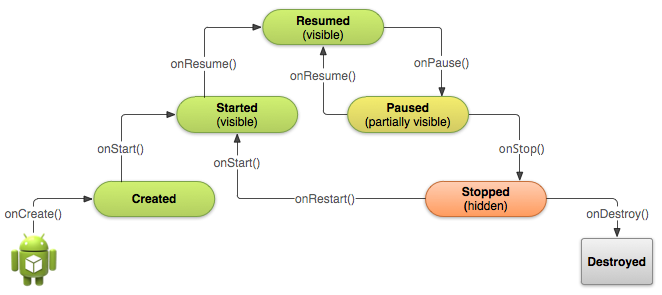
\includegraphics[width=0.95\linewidth]{figuras/estados}
	\caption{Ciclo de una actividad}
	\label{fig:estados}
\end{figure}


\subsection{Recursos de las aplicaciones Android }
 
Una aplicación para Android se compone de algo más que código, requiere de recursos que están separados, como imágenes, archivos de audio, y todo lo relativo a la presentación visual de la aplicación.

Para todos estos recursos Android proporciona un identificador único entero dentro de la aplicación, que puede utilizarse para hacer referencia al recurso en el código de aplicación o de otros recursos definidos en XML. 
Hay distintos tipos de recursos, que se definen en ficheros XML alojados en una cierta subcarpeta de res: 

\begin{itemize}	

	\item \emph{\textbf{Valores simples \textit{(carpeta values)}: }}  Strings, colores y dimensiones. Cada fichero XML contiene la definición de uno o más de estos elementos. Todos estos recursos se identifican con el valor de su atributo name. 
	
	\item \emph{\textbf{Recursos dibujables\textit{(carpeta drawable)}: }} Ficheros con imágenes, incluyendo el icono de la aplicación. Estos recursos se identifican con su nombre de fichero, y los recuadros de color con el valor de su atributo name.
	 
	\item \emph{\textbf{Animaciones\textit{(carpeta anim)}: }} Usados para animaciones sencillas sobre uno o varios gráficos: rotaciones. Fading, movimiento, etc. Cada animación se define en un fichero xML. Se identifican con su nombre de fichero. 
	
	\item \emph{\textbf{menu\textit{(carpeta menu)}: }}  Existen tres tipos de menús: de opciones, contextual y submenú. El menú de opciones y el menú contextual se identifican con su nombre de fichero y el submenú con el valor de su atributo id. 
	
	\item \emph{\textbf{Diseños\textit{(carpeta layout)}: }}  Cada layout se define en un fichero XML. Dentro del layout se definen los elementos que lo componen, como puedan ser los Views o los ViewGroups. Se identificará por su nombre de fichero y los elementos del layout se podrán identificar con su atributo id. 
	
	\item \emph{\textbf{Estilos\textit{(carpeta values)}: }} Un estilo es uno o más atributos que se aplican a un elemento. El tema se define como uno o más atributos que se aplican a todo lo que hay en pantalla, este se asigna como atributo a una actividad en el Manifiesto. El estilo se referencia con el valor de su atributo name.  
					
\end{itemize}

También existen otros recursos como drawables, internacionalización, etc.




